\section*{Constitutive Properties and Gait Integration}

\subsection*{Gait Cycle Integration and Stimulus Accumulation}
The daily mechanical stimulus $\psi_{\mathrm{day}}$ aggregates the loading history over a full day. In our numerical experiments, the gait cycle is represented by a finite set of loading cases (phases) with relative daily frequencies $c_i$, and the daily driver is computed as the cycle-weighted power mean in \eqref{eq:stim-psi-nd}. The exponent $p$ plays a critical role in filtering the mechanical signal: $p=1$ gives a weighted mean, while larger $p$ increasingly biases toward peak loads ($p\to\infty$ approaches a max). Under linear elasticity $\psi_i\propto F^2$, so the power kernel scales as $F^{2p}$ and convexity (Jensen’s inequality) explains why dynamic peaks produce a stronger stimulus than a constant load of equivalent average magnitude.

\begin{figure}[htbp]
    \centering
    \IfFileExists{images/gait_driver_analysis.png}{%
        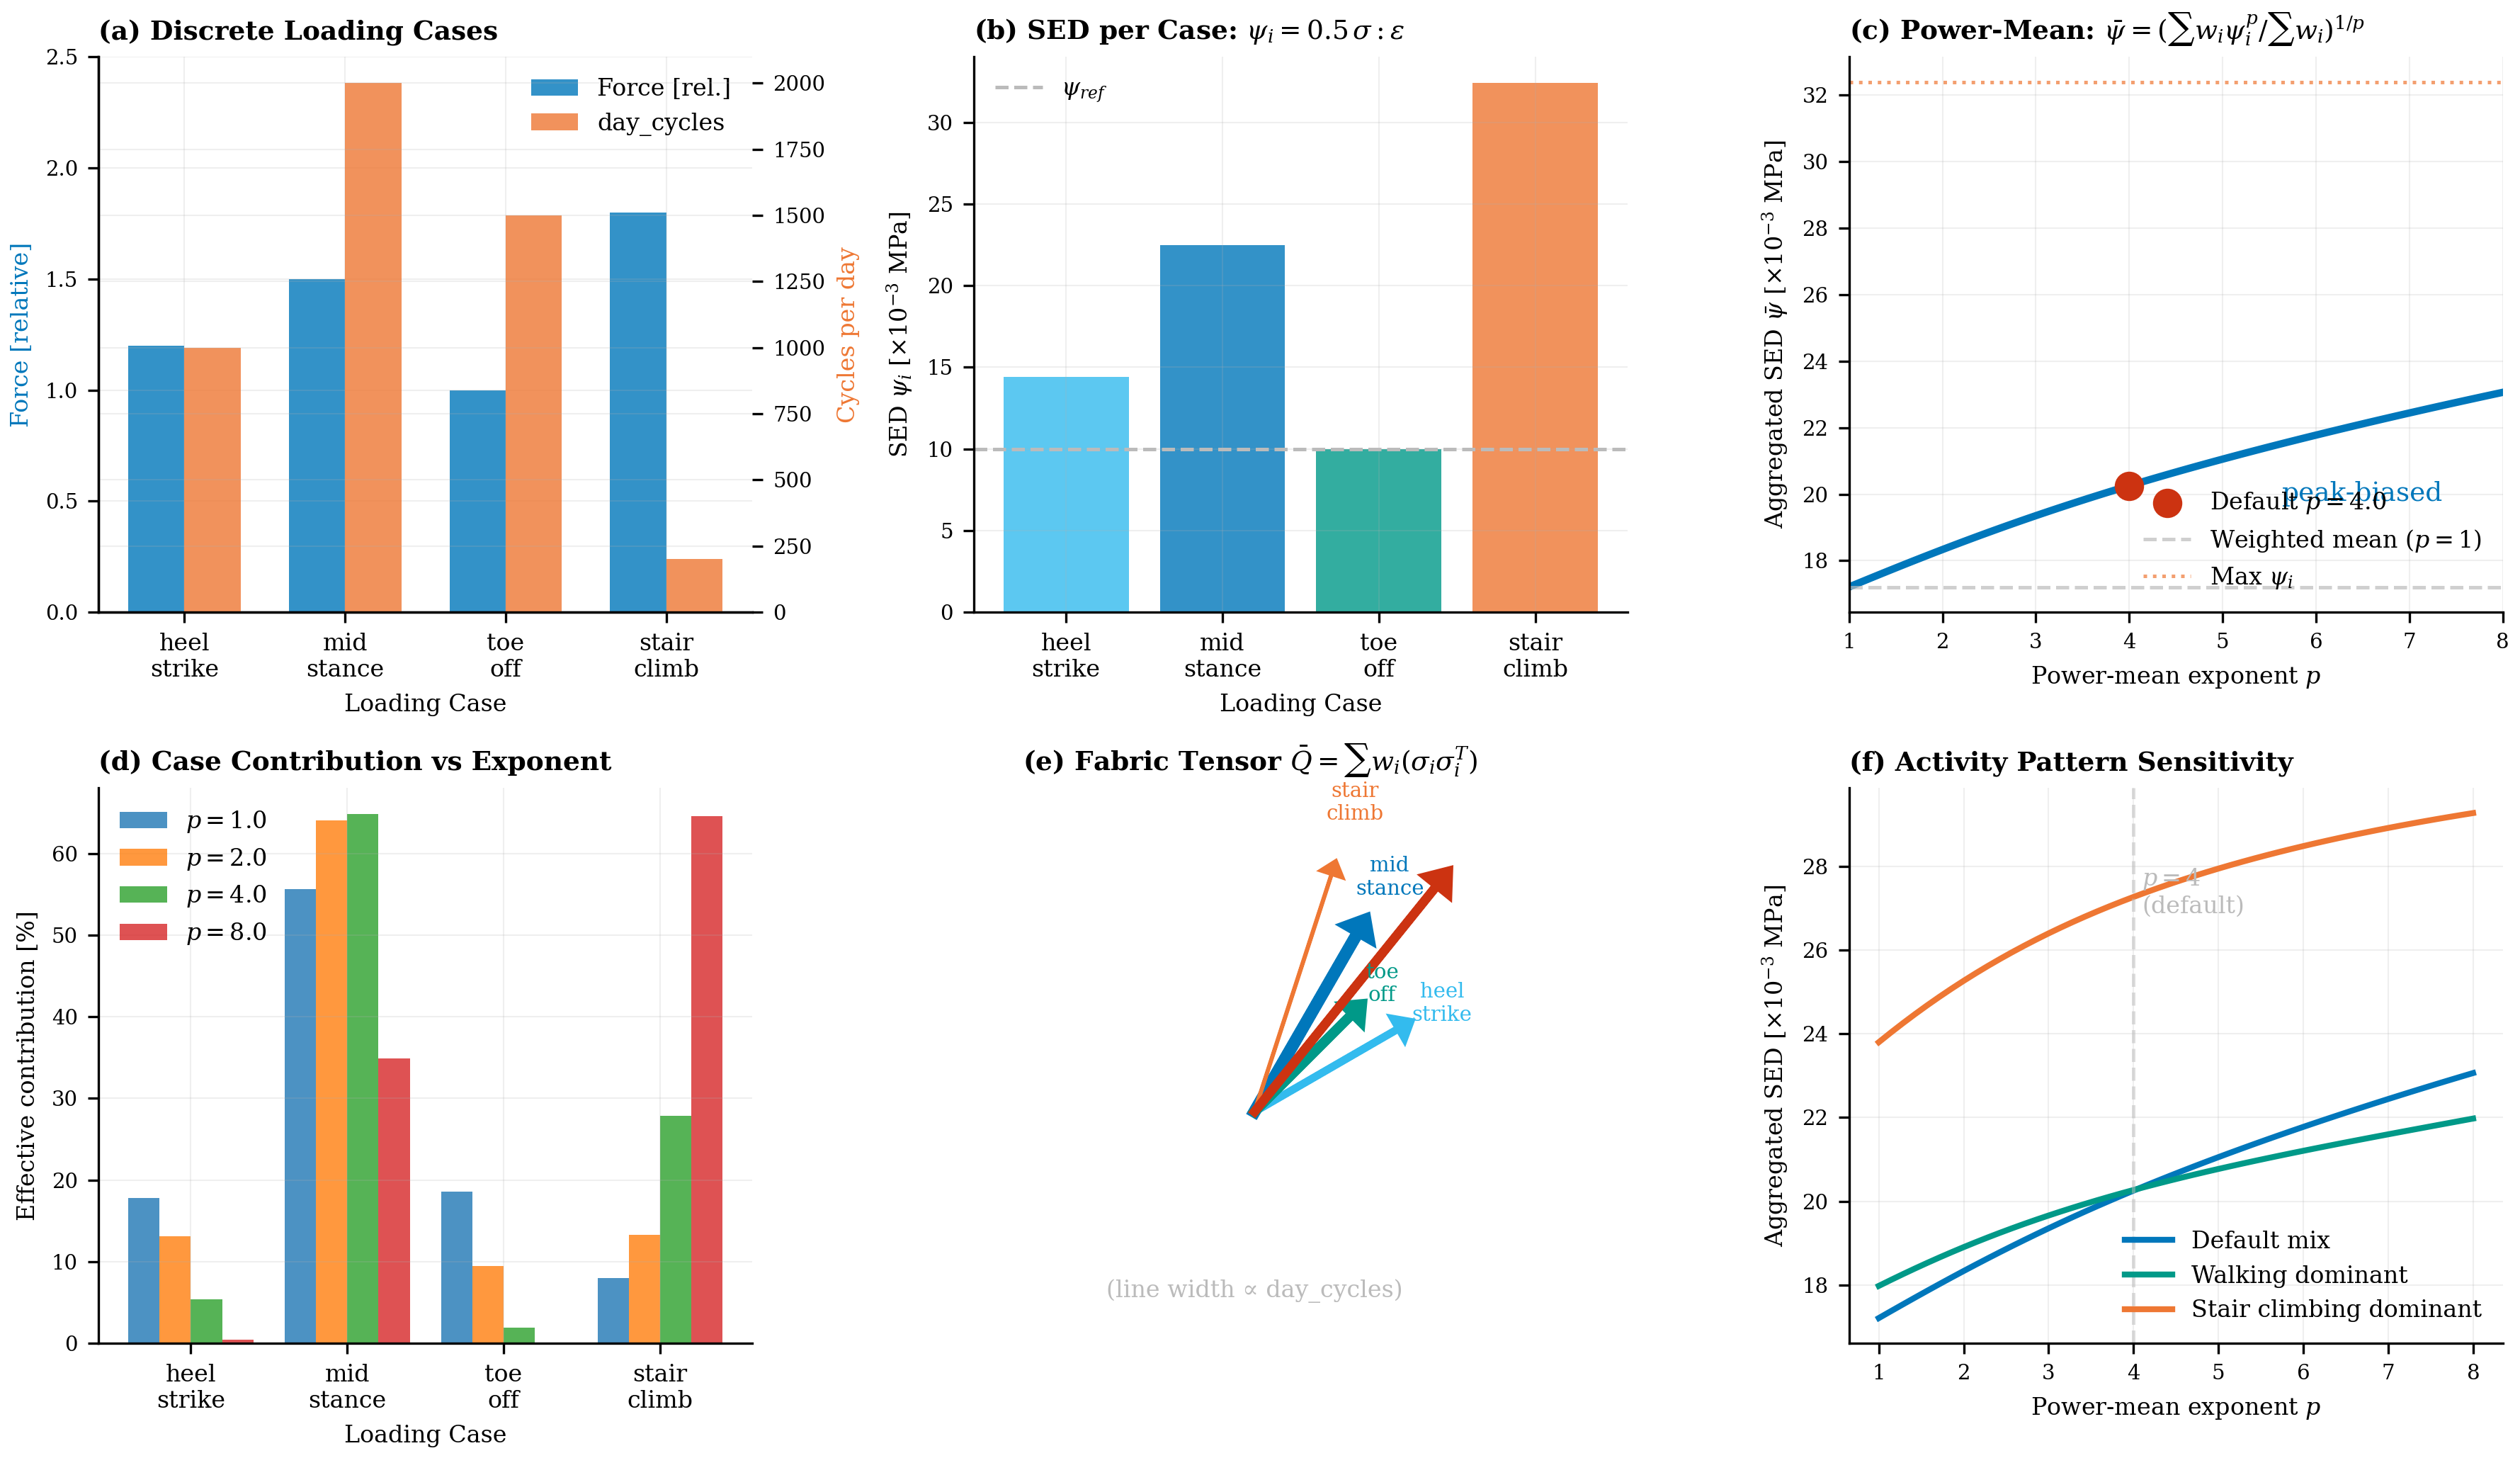
\includegraphics[width=\textwidth]{images/gait_driver_analysis.png}%
    }{\fbox{\parbox{0.9\linewidth}{\centering Missing image: \texttt{images/gait\_driver\_analysis.png}}}}
    \caption{Gait stimulus aggregation. (A) Representative hip contact force profile normalized to body weight (BW), showing characteristic heel-strike and toe-off peaks. (B) Instantaneous power kernel $(U/U_{\mathrm{ref}})^p$ for varying exponents $p$ (power-mean bias). Since $U \propto F^2$, the signal scales as $F^{2p}$, strongly amplifying peak loads as $p$ increases. (C) The cycle-averaged amplification factor versus $p$.}
    \label{fig:gait_stimulus}
\end{figure}

Figure \ref{fig:gait_stimulus} illustrates this effect using a synthetic hip contact force profile. Panel (B) demonstrates how the instantaneous kernel sharpens around peaks as $p$ increases. Panel (C) compares the cycle-averaged amplification for a dynamic gait load versus a constant load of equivalent average magnitude.

